% Options for packages loaded elsewhere
\PassOptionsToPackage{unicode}{hyperref}
\PassOptionsToPackage{hyphens}{url}
\PassOptionsToPackage{dvipsnames,svgnames,x11names}{xcolor}
%
\documentclass[
  letterpaper,
  DIV=11,
  numbers=noendperiod]{scrreprt}

\usepackage{amsmath,amssymb}
\usepackage{iftex}
\ifPDFTeX
  \usepackage[T1]{fontenc}
  \usepackage[utf8]{inputenc}
  \usepackage{textcomp} % provide euro and other symbols
\else % if luatex or xetex
  \usepackage{unicode-math}
  \defaultfontfeatures{Scale=MatchLowercase}
  \defaultfontfeatures[\rmfamily]{Ligatures=TeX,Scale=1}
\fi
\usepackage{lmodern}
\ifPDFTeX\else  
    % xetex/luatex font selection
\fi
% Use upquote if available, for straight quotes in verbatim environments
\IfFileExists{upquote.sty}{\usepackage{upquote}}{}
\IfFileExists{microtype.sty}{% use microtype if available
  \usepackage[]{microtype}
  \UseMicrotypeSet[protrusion]{basicmath} % disable protrusion for tt fonts
}{}
\makeatletter
\@ifundefined{KOMAClassName}{% if non-KOMA class
  \IfFileExists{parskip.sty}{%
    \usepackage{parskip}
  }{% else
    \setlength{\parindent}{0pt}
    \setlength{\parskip}{6pt plus 2pt minus 1pt}}
}{% if KOMA class
  \KOMAoptions{parskip=half}}
\makeatother
\usepackage{xcolor}
\usepackage{svg}
\setlength{\emergencystretch}{3em} % prevent overfull lines
\setcounter{secnumdepth}{5}
% Make \paragraph and \subparagraph free-standing
\ifx\paragraph\undefined\else
  \let\oldparagraph\paragraph
  \renewcommand{\paragraph}[1]{\oldparagraph{#1}\mbox{}}
\fi
\ifx\subparagraph\undefined\else
  \let\oldsubparagraph\subparagraph
  \renewcommand{\subparagraph}[1]{\oldsubparagraph{#1}\mbox{}}
\fi


\providecommand{\tightlist}{%
  \setlength{\itemsep}{0pt}\setlength{\parskip}{0pt}}\usepackage{longtable,booktabs,array}
\usepackage{calc} % for calculating minipage widths
% Correct order of tables after \paragraph or \subparagraph
\usepackage{etoolbox}
\makeatletter
\patchcmd\longtable{\par}{\if@noskipsec\mbox{}\fi\par}{}{}
\makeatother
% Allow footnotes in longtable head/foot
\IfFileExists{footnotehyper.sty}{\usepackage{footnotehyper}}{\usepackage{footnote}}
\makesavenoteenv{longtable}
\usepackage{graphicx}
\makeatletter
\def\maxwidth{\ifdim\Gin@nat@width>\linewidth\linewidth\else\Gin@nat@width\fi}
\def\maxheight{\ifdim\Gin@nat@height>\textheight\textheight\else\Gin@nat@height\fi}
\makeatother
% Scale images if necessary, so that they will not overflow the page
% margins by default, and it is still possible to overwrite the defaults
% using explicit options in \includegraphics[width, height, ...]{}
\setkeys{Gin}{width=\maxwidth,height=\maxheight,keepaspectratio}
% Set default figure placement to htbp
\makeatletter
\def\fps@figure{htbp}
\makeatother
% definitions for citeproc citations
\NewDocumentCommand\citeproctext{}{}
\NewDocumentCommand\citeproc{mm}{%
  \begingroup\def\citeproctext{#2}\cite{#1}\endgroup}
\makeatletter
 % allow citations to break across lines
 \let\@cite@ofmt\@firstofone
 % avoid brackets around text for \cite:
 \def\@biblabel#1{}
 \def\@cite#1#2{{#1\if@tempswa , #2\fi}}
\makeatother
\newlength{\cslhangindent}
\setlength{\cslhangindent}{1.5em}
\newlength{\csllabelwidth}
\setlength{\csllabelwidth}{3em}
\newenvironment{CSLReferences}[2] % #1 hanging-indent, #2 entry-spacing
 {\begin{list}{}{%
  \setlength{\itemindent}{0pt}
  \setlength{\leftmargin}{0pt}
  \setlength{\parsep}{0pt}
  % turn on hanging indent if param 1 is 1
  \ifodd #1
   \setlength{\leftmargin}{\cslhangindent}
   \setlength{\itemindent}{-1\cslhangindent}
  \fi
  % set entry spacing
  \setlength{\itemsep}{#2\baselineskip}}}
 {\end{list}}
\usepackage{calc}
\newcommand{\CSLBlock}[1]{\hfill\break\parbox[t]{\linewidth}{\strut\ignorespaces#1\strut}}
\newcommand{\CSLLeftMargin}[1]{\parbox[t]{\csllabelwidth}{\strut#1\strut}}
\newcommand{\CSLRightInline}[1]{\parbox[t]{\linewidth - \csllabelwidth}{\strut#1\strut}}
\newcommand{\CSLIndent}[1]{\hspace{\cslhangindent}#1}

\KOMAoption{captions}{tableheading}
\makeatletter
\@ifpackageloaded{tcolorbox}{}{\usepackage[skins,breakable]{tcolorbox}}
\@ifpackageloaded{fontawesome5}{}{\usepackage{fontawesome5}}
\definecolor{quarto-callout-color}{HTML}{909090}
\definecolor{quarto-callout-note-color}{HTML}{0758E5}
\definecolor{quarto-callout-important-color}{HTML}{CC1914}
\definecolor{quarto-callout-warning-color}{HTML}{EB9113}
\definecolor{quarto-callout-tip-color}{HTML}{00A047}
\definecolor{quarto-callout-caution-color}{HTML}{FC5300}
\definecolor{quarto-callout-color-frame}{HTML}{acacac}
\definecolor{quarto-callout-note-color-frame}{HTML}{4582ec}
\definecolor{quarto-callout-important-color-frame}{HTML}{d9534f}
\definecolor{quarto-callout-warning-color-frame}{HTML}{f0ad4e}
\definecolor{quarto-callout-tip-color-frame}{HTML}{02b875}
\definecolor{quarto-callout-caution-color-frame}{HTML}{fd7e14}
\makeatother
\makeatletter
\@ifpackageloaded{bookmark}{}{\usepackage{bookmark}}
\makeatother
\makeatletter
\@ifpackageloaded{caption}{}{\usepackage{caption}}
\AtBeginDocument{%
\ifdefined\contentsname
  \renewcommand*\contentsname{Table of contents}
\else
  \newcommand\contentsname{Table of contents}
\fi
\ifdefined\listfigurename
  \renewcommand*\listfigurename{List of Figures}
\else
  \newcommand\listfigurename{List of Figures}
\fi
\ifdefined\listtablename
  \renewcommand*\listtablename{List of Tables}
\else
  \newcommand\listtablename{List of Tables}
\fi
\ifdefined\figurename
  \renewcommand*\figurename{Figure}
\else
  \newcommand\figurename{Figure}
\fi
\ifdefined\tablename
  \renewcommand*\tablename{Table}
\else
  \newcommand\tablename{Table}
\fi
}
\@ifpackageloaded{float}{}{\usepackage{float}}
\floatstyle{ruled}
\@ifundefined{c@chapter}{\newfloat{codelisting}{h}{lop}}{\newfloat{codelisting}{h}{lop}[chapter]}
\floatname{codelisting}{Listing}
\newcommand*\listoflistings{\listof{codelisting}{List of Listings}}
\makeatother
\makeatletter
\makeatother
\makeatletter
\@ifpackageloaded{caption}{}{\usepackage{caption}}
\@ifpackageloaded{subcaption}{}{\usepackage{subcaption}}
\makeatother
\ifLuaTeX
  \usepackage{selnolig}  % disable illegal ligatures
\fi
\usepackage{bookmark}

\IfFileExists{xurl.sty}{\usepackage{xurl}}{} % add URL line breaks if available
\urlstyle{same} % disable monospaced font for URLs
\hypersetup{
  pdftitle={Decision Making with Statistics},
  pdfauthor={Guillaume Gilles},
  colorlinks=true,
  linkcolor={blue},
  filecolor={Maroon},
  citecolor={Blue},
  urlcolor={Blue},
  pdfcreator={LaTeX via pandoc}}

\title{Decision Making with Statistics}
\usepackage{etoolbox}
\makeatletter
\providecommand{\subtitle}[1]{% add subtitle to \maketitle
  \apptocmd{\@title}{\par {\large #1 \par}}{}{}
}
\makeatother
\subtitle{MS04-001-G}
\author{Guillaume Gilles}
\date{2024-01-15}

\begin{document}
\maketitle

\renewcommand*\contentsname{Table of contents}
{
\hypersetup{linkcolor=}
\setcounter{tocdepth}{2}
\tableofcontents
}
\bookmarksetup{startatroot}

\chapter{Decision Making with
Statistics}\label{decision-making-with-statistics}

MS04-001-G

\hfill\break

This is a Quarto book.

To learn more about Quarto books visit
\url{https://quarto.org/docs/books}.

https://quarto.org/docs/books/book-structure.html: This page should
include the preface, acknowledgements, etc. and headings in the
index.qmd file are unnumbered by default. The HTML version of the book
will use the index.qmd as the home page and if provided, will place the
cover-image on that page.

The references.qmd file will include the generated bibliography (see
References below for details).

The syllabus can be found \href{syllabus.qmd}{here}

\begin{itemize}
\tightlist
\item[$\square$]
  Embedding khan academy video at the end of each section
\item[$\square$]
  folded table of content on first level
\item[$\square$]
  insert link (cross reference) between figure. par dans les random
  variable quand on parle des combination cf! calculation of
  probabilities
\item[$\square$]
  processus stochastic miage
\item[$\square$]
  openclassroom proba / stat
\item[$\square$]
  kassie kozolov: medium, youtube, etc.
\end{itemize}

\section{Calculation of
probabilities}\label{calculation-of-probabilities}

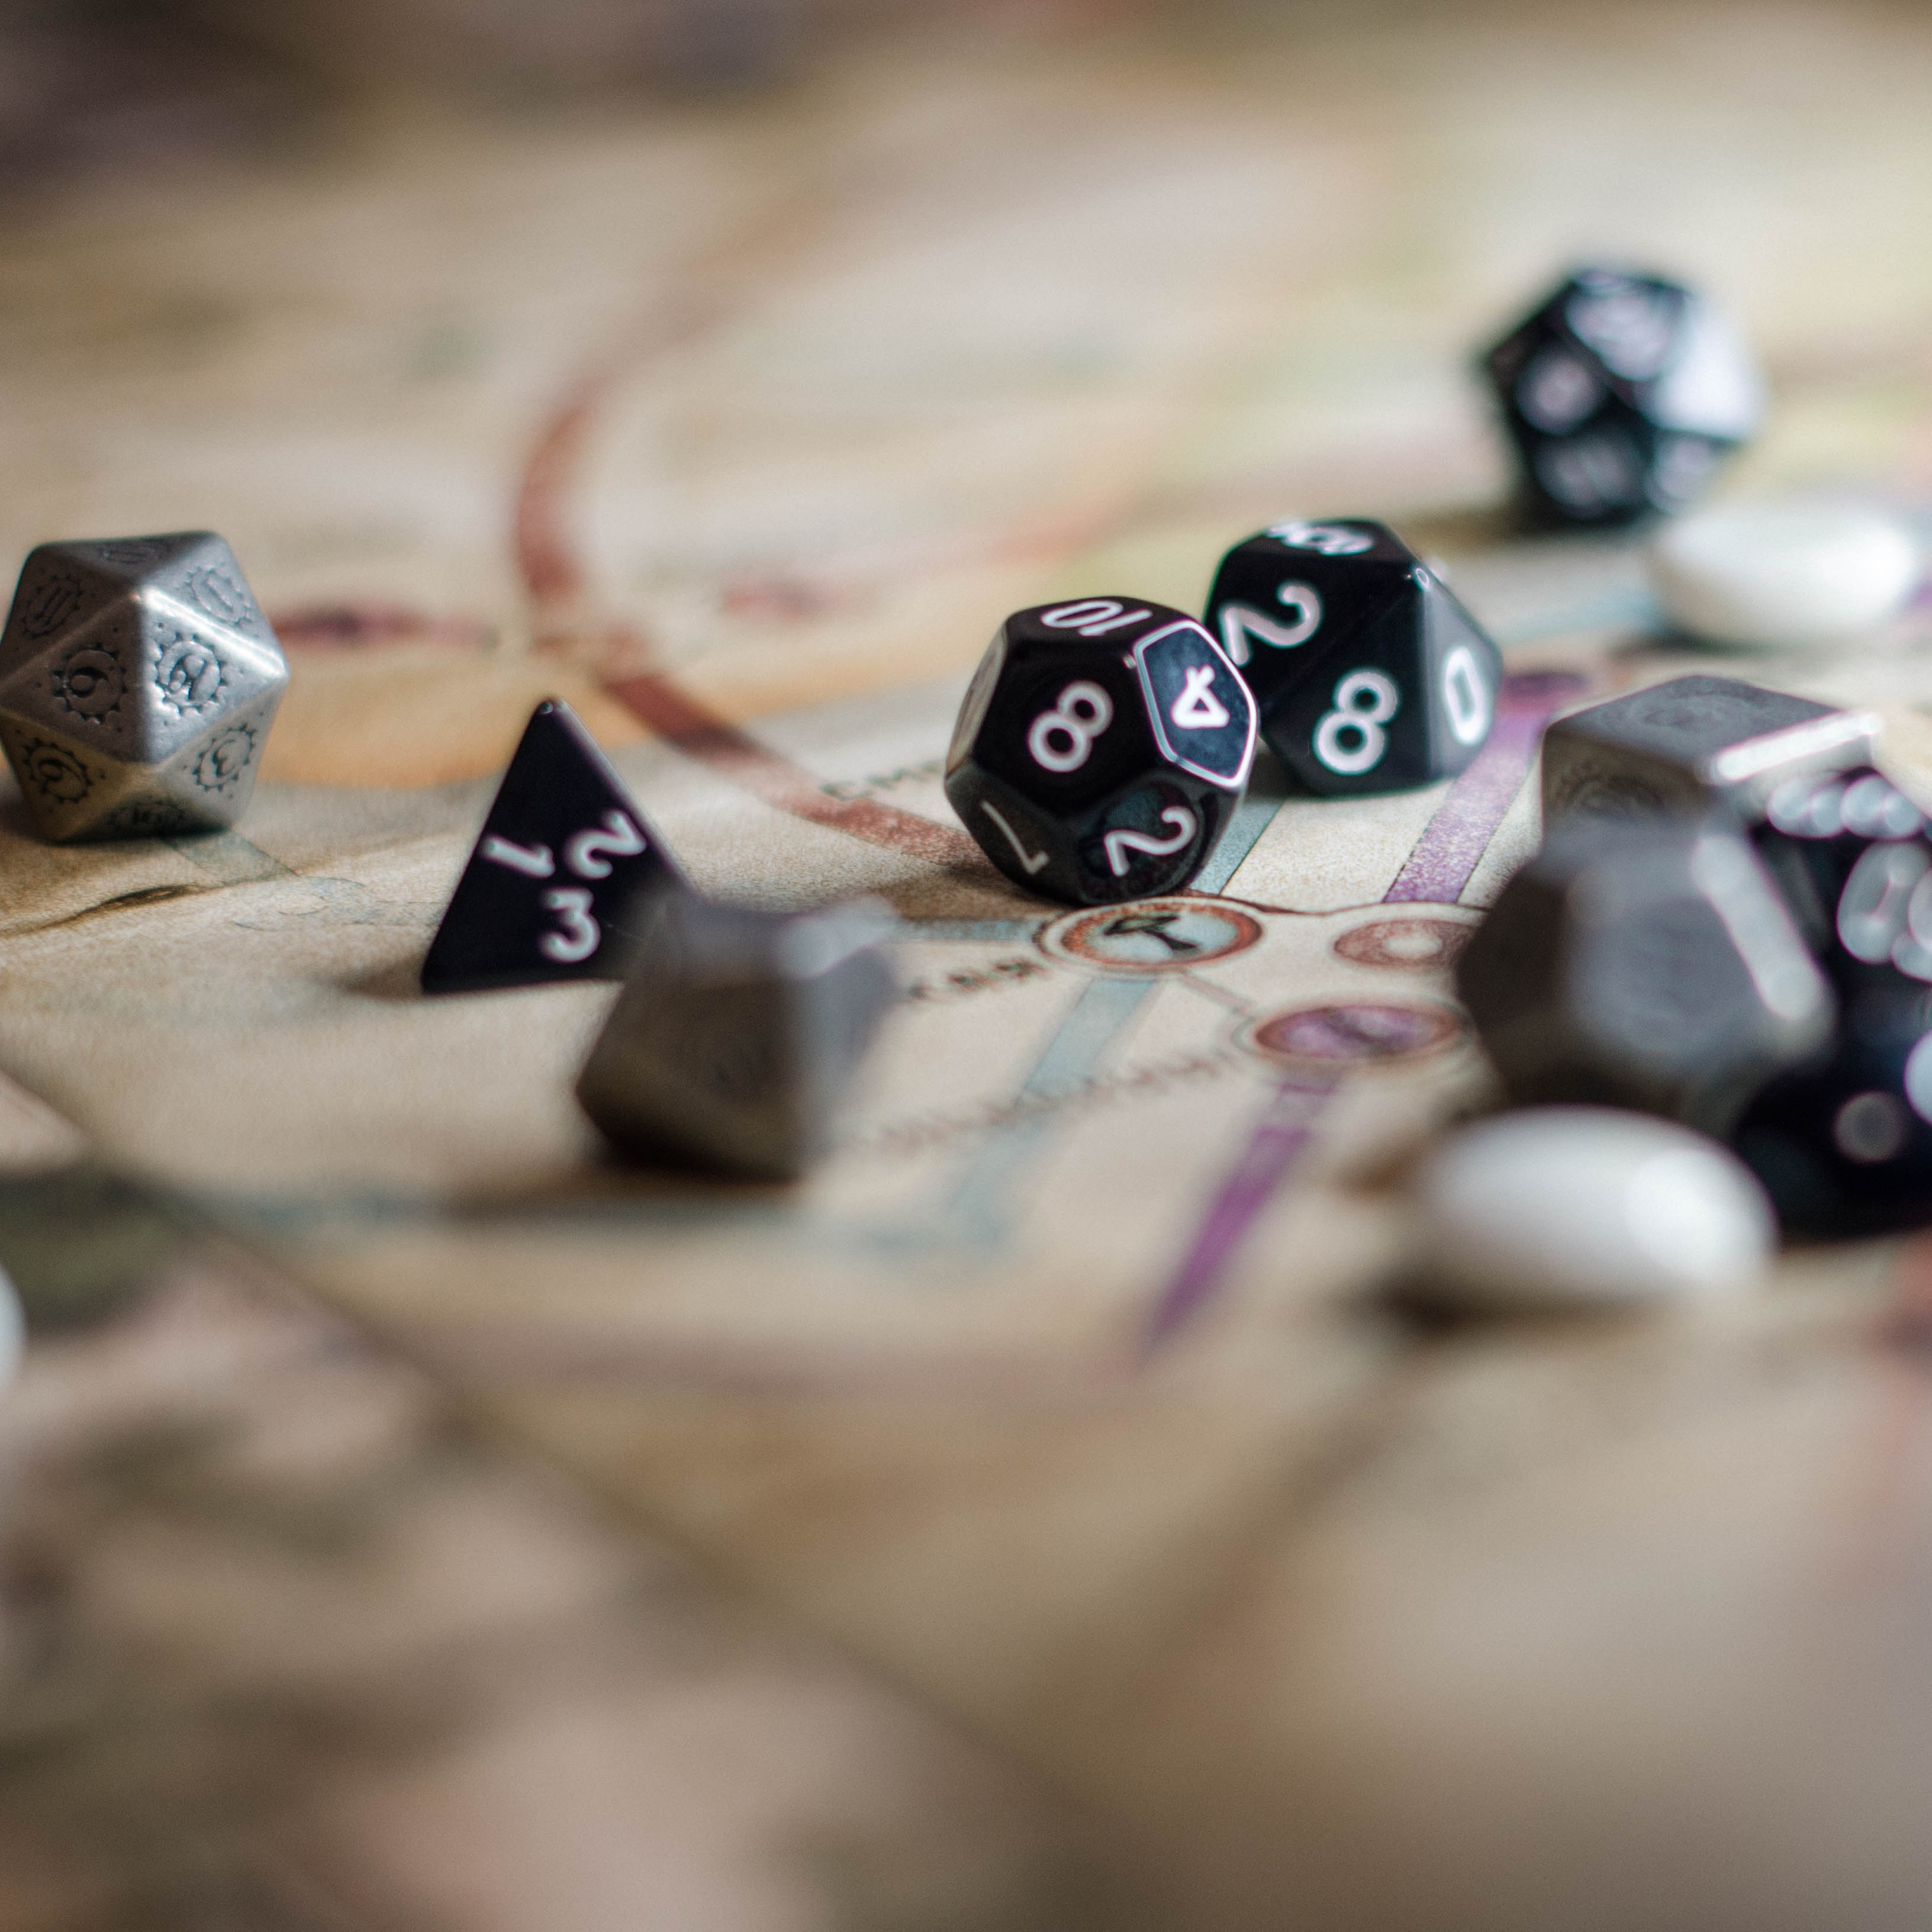
\includegraphics{../img/dice_map.jpg}

Practical approach: Probability allows to measure the likelihood of an
event. Some definitions : Random experiment: an experiment (involving
chance) whose results can not be predicted with certainty Universe: the
set of all possible outcomes of a random experiment, noted Ω Event: a
part or subset of the universe

Probability: a number between 0 and 1 that gives a measure of the
likelihood of an event. In other words, if 𝐸 is an event, then

0 ≤ ℙ(𝐸) ≤ 1 Special cases of events: Certain event: it can be described
with all the elements of Ω and in that case its probability is 1
Impossible event: there exist no element of Ω which can describe it and
in that case its probability is 0

Properties and basic operations:

Inclusion : 𝐴 ⊂ 𝐵 ⇒ ℙ(𝐴) ≤ ℙ(𝐵) Intersection : ℙ(𝐴 ∩ 𝐵) ≤ ℙ(𝐵) and ℙ(𝐴 ∩
𝐵) ≤ ℙ(𝐴) If ℙ(𝐴 ∩ 𝐵) = ℙ(𝐴) × ℙ(𝐵), then 𝐴 and 𝐵 are two independent
events If 𝐴 and 𝐵 are disjoint (i.e.~𝐴 ∩ 𝐵 = ∅ ), then ℙ(𝐴 ∩ 𝐵) = 0

Union : ℙ (𝐴)≤ℙ(𝐴∪𝐵), ℙ(𝐵) ≤ ℙ(𝐴∪𝐵) and ℙ(𝐴∩𝐵) ≤ ℙ(𝐴∪𝐵) ℙ(𝐴 ∪ 𝐵)= ℙ(𝐴)+
ℙ(𝐵)− ℙ(𝐴 ∩ 𝐵) Therefore, if 𝐴 and 𝐵 are two disjoint events, then ℙ(𝐴 ∪
𝐵) = ℙ(𝐴) + ℙ(𝐵) The difference : (𝐴∖𝐵) ⊂ 𝐴 ⇒ ℙ(𝐴∖𝐵) ≤ ℙ(𝐴) ℙ(𝐴∖𝐵) =
ℙ(𝐴) − ℙ(𝐴 ∩ 𝐵) If 𝐴 and 𝐵 are two disjoint events, then (𝐴∖𝐵) = 𝐴.
Therefore, one gets ℙ(𝐴∖𝐵) = ℙ(𝐴).

Complementarity : The complement of the event 𝐴 is an event (denoted 𝐴~̅
or Ω∖𝐴) that contains all elements of Ω not belonging to 𝐴

\[P(\overline{A}) = 1 - P(A)\]

Equiprobability

Assume that the universe \(\Omega\) of a random experiment is a finite
set. We talk of equiprobability when all the possible outcomes of the
experiment have the same probability (of realization). Let \(A\) be an
event associated with this experiment. In that case, we have:

\[P(𝐴) = \frac{\text{Number of favorable cases}}{\text{Number of possible cases}}\]

The conditional probability

Let \(A\) and \(B\), two events from the same universe \(\Omega\).
Suppose that \(A\) is a non-zero probability event. We call
\textbf{conditional probability} of \(B\) such \(A\) (or knowing that
\(A\) is realized) the quantity defined as follows:

\[P(B \vert A) = \frac{P(A \cap B)}{P(A)}\]

In the same way, the conditional probability of \(A\) such \(B\) (or
knowing that \(B\) is realized) is defined by:

\[P(A \vert B) = \frac{P(A \cap B)}{P(B)}\]

If \(A\) and \(B\) are two independent events, then:

\[P(A \vert B) = P(𝐴)\]

\[P(B \vert A) = P(B)\]

Total Probability Formula:

Let \(\{𝐸1, ..., 𝐸_𝑘\}\) be a partition of \(\Omega\) (such that 𝐸\_𝑖 ≠
∅ for all 𝑖 = 1,\ldots,𝑘) Let 𝐵 be an event. We have :

``ℙ'' (𝐵)= ∑\_(𝑖=1)\^{}𝑘▒``ℙ'' (𝐵∩𝐸\_𝑖 )

\begin{verbatim}
                 =∑_(𝑖=1)^𝑘▒〖"ℙ" (𝐸_𝑖 )" ℙ" (𝐵 ┤| 𝐸_𝑖)〗
\end{verbatim}

\section{Sets and Combinatorial
Analysis}\label{sets-and-combinatorial-analysis}

\begin{itemize}
\tightlist
\item
  \href{https://en.wikipedia.org/wiki/Set_(mathematics)\#cite_ref-Cantor_1-0}{wikipedia
  page}
\item
  \href{https://www.khanacademy.org/math/statistics-probability/probability-library/basic-set-ops/v/intersection-and-union-of-sets}{Basic
  set operations}
\item
  \href{https://www.khanacademy.org/math/statistics-probability/counting-permutations-and-combinations}{Unit
  8: Counting, permutations, and combinations}
\item
  \href{https://r-graph-gallery.com/venn-diagram.html}{Venn Diagram}
\end{itemize}

\subsection{Definition}\label{definition}

A set is the mathematical model for a collection of different and
distinct \textbf{things} / \textbf{objects} ; a set contains elements or
members, which can be mathematical objects of any kind: numbers,
symbols, points in space, lines, other geometrical shapes, variables, or
even other sets. The set with no elements is the empty set; a set with a
single element is a singleton. A set may have a finite number of
elements or be an infinite set.

Definitions : A set 𝐸 is a collection of objects, called its elements,
considered \textbf{without order} or \textbf{possible repetition} (parce
que ce sont des objets). If '' 𝑥 is an element of the set 𝐸 ``, then one
can say that''𝑥 belongs to 𝐸 '' and we denote 𝑥 ∈ 𝐸 A set without
element is called empty set: notation: ∅ A single-element set is called
a singleton A two-element set, is called a pair A subset is a part of
the set

\subsection{How to represent a set}\label{how-to-represent-a-set}

Representation of a set : By extension: give an exhaustive list of all
its elements. By understanding: give a characteristic property of its
elements. For example : 𝐴 = \{𝑥 ∈ℕ ┤\textbar{} x is an even number\} by
extension : 𝐴 = \{0, 2, 4, 6, 8,\ldots\} 𝐵 = \{𝑥 ∈ℤ \textbar{} −2 ≤ 𝑥 ≤
5\} by extension : 𝐵 = \{−2,−1, 0, 1, 2, 3, 4, 5\}

\subsection{Usual sets in mathematics}\label{usual-sets-in-mathematics}

Usual sets in mathematics : ℕ'' = \{0, 1, 2, 3, 4, . . .\} ``the set of
nonnegative integers ℤ'' = \{\ldots, −2, −1, 0, 1, 2, \ldots\}'' the set
of integers ℚ=\{ 𝑎/𝑏, 𝑎∈ℤ, 𝑏∈ℤ, and 𝑏≠0\} the set of rational numbers
(the fractions) ℝ ``= {]}−∞, +∞{[}'' the set of real numbers ℝ
``~''\{𝑎\} the set of all the real numbers in ℝ except 𝑎 ℝ\^{}+ ``=
{[}0, +∞{[}'' the set of positif real numbers ℝ\^{}− ''= {]}−∞, 0{]}''
the set of negatif real numbers

\subsection{Operations on sets}\label{operations-on-sets}

Operations on Sets :

\subsubsection{Inclusion : 𝐴 ⊂ 𝐵 :}\label{inclusion-ux1d434-ux1d435}

∀ 𝑥∈𝐴 ⇒ 𝑥∈𝐵

\subsubsection{Equality : 𝐴 = 𝐵}\label{equality-ux1d434-ux1d435}

∀ 𝑥∈𝐴 ⟺𝑥∈𝐵

Note that 𝐴 ⊆ 𝐵 implies '' 𝐴 is included in 𝐵 or equal to 𝐵 ``.

Recall that : 𝐴=𝐵 ⟺ 𝐴⊆𝐵 and 𝐵⊆𝐴.

\subsubsection{Intersection : 𝐴 ∩ 𝐵}\label{intersection-ux1d434-ux1d435}

∀ 𝑥 ∈ 𝐴 ∩ 𝐵⟺𝑥 ∈ 𝐴 and 𝑥 ∈ 𝐵.

Recall that : if 𝐴∩𝐵=∅, then one can say that 𝐴 and 𝐵 are disjoint 𝐴∩𝐵 =
𝐵∩𝐴 𝐴∩∅ = ∅ 𝐴∩(𝐵∩𝐶) = (𝐴∩𝐵)∩𝐶

\subsubsection{Union : 𝐴∪𝐵}\label{union-ux1d434ux1d435}

∀ 𝑥 ∈𝐴∪𝐵⟺𝑥 ∈ 𝐴 or 𝑥 ∈ 𝐵.

\begin{verbatim}
Recall that :
\end{verbatim}

𝐴⊆(𝐴∪𝐵),𝐵⊆(𝐴∪𝐵),and 𝐴∩𝐵⊆(𝐴∪𝐵) 𝐴∪𝐵=𝐵∪𝐴 𝐴∪∅=𝐴 𝐴∪(𝐵∪𝐶)=(𝐴∪𝐵)∪𝐶
𝐴∩(𝐵∪𝐶)=(𝐴∩𝐵)∪(𝐴∩𝐶)

\subsubsection{Complementarity : Let 𝐴, 𝐵 and 𝐶 be three sets, such that
𝐴 ⊂ 𝐵 and 𝐶⊂ 𝐵. The complement of 𝐴 in 𝐵 is the set of elements of 𝐵 not
belonging to
𝐴.}\label{complementarity-let-ux1d434-ux1d435-and-ux1d436-be-three-sets-such-that-ux1d434-ux1d435-and-ux1d436-ux1d435.-the-complement-of-ux1d434-in-ux1d435-is-the-set-of-elements-of-ux1d435-not-belonging-to-ux1d434.}

\begin{verbatim}
Notation :  𝐴 ̅  (or 𝐴^𝑐, or 𝐵∖𝐴). 
\end{verbatim}

Recall that : A ∩ 𝐴~̅ = ∅ A ∪ 𝐴~̅ = B ((𝐴~̅))~̅ = A ((𝐴∩𝐶))~̅ = 𝐴~̅ ∪ 𝐶~̅ and
((𝐴 ∪ 𝐶) )~̅ = 𝐴~̅ ∩ 𝐶~̅

🏁🏁

\section{Calculation of
probabilities}\label{calculation-of-probabilities-1}

\begin{itemize}
\tightlist
\item
  \href{https://openclassrooms.com/fr/courses/4525296-maitrisez-les-bases-des-probabilites}{Maîtrisez
  les bases des probabilités}
\end{itemize}

🏁🏁

\bookmarksetup{startatroot}

\chapter{Sets and Combinatorial
Analysis}\label{sets-and-combinatorial-analysis-1}

\section{Set}\label{set}

Definitions : A set 𝐸 is a collection of objects, called its elements,
considered without order or possible repetition. If '' 𝑥 is an element
of the set 𝐸 ``, then one can say that''𝑥 belongs to 𝐸 '' and we denote
𝑥 ∈ 𝐸 A set without element is called empty set: notation: ∅ A
single-element set is called a singleton A two-element set, is called a
pair A subset is a part of the set

Usual sets in mathematics : ℕ'' = \{0, 1, 2, 3, 4, . . .\} ``the set of
nonnegative integers ℤ'' = \{\ldots, −2, −1, 0, 1, 2, \ldots\}'' the set
of integers ℚ=\{ 𝑎/𝑏, 𝑎∈ℤ, 𝑏∈ℤ, and 𝑏≠0\} the set of rational numbers
(the fractions) ℝ ``= {]}−∞, +∞{[}'' the set of real numbers ℝ
``~''\{𝑎\} the set of all the real numbers in ℝ except 𝑎 ℝ\^{}+ ``=
{[}0, +∞{[}'' the set of positif real numbers ℝ\^{}− ''= {]}−∞, 0{]}''
the set of negatif real numbers

Representation of a set : By extension: give an exhaustive list of all
its elements. By understanding: give a characteristic property of its
elements. For example : 𝐴 = \{𝑥 ∈ℕ ┤\textbar{} x is an even number\} by
extension : 𝐴 = \{0, 2, 4, 6, 8,\ldots\} 𝐵 = \{𝑥 ∈ℤ \textbar{} −2 ≤ 𝑥 ≤
5\} by extension : 𝐵 = \{−2,−1, 0, 1, 2, 3, 4, 5\}

Operations on Sets : Inclusion : 𝐴 ⊂ 𝐵 : ∀ 𝑥∈𝐴 ⇒ 𝑥∈𝐵

Equality : 𝐴 = 𝐵 ∀ 𝑥∈𝐴 ⟺𝑥∈𝐵

Note that 𝐴 ⊆ 𝐵 implies '' 𝐴 is included in 𝐵 or equal to 𝐵 ``.

Recall that : 𝐴=𝐵 ⟺ 𝐴⊆𝐵 and 𝐵⊆𝐴.

Intersection : 𝐴 ∩ 𝐵 ∀ 𝑥 ∈ 𝐴 ∩ 𝐵⟺𝑥 ∈ 𝐴 and 𝑥 ∈ 𝐵.

Recall that : if 𝐴∩𝐵=∅, then one can say that 𝐴 and 𝐵 are disjoint 𝐴∩𝐵 =
𝐵∩𝐴 𝐴∩∅ = ∅ 𝐴∩(𝐵∩𝐶) = (𝐴∩𝐵)∩𝐶

Union : 𝐴∪𝐵 ∀ 𝑥 ∈𝐴∪𝐵⟺𝑥 ∈ 𝐴 or 𝑥 ∈ 𝐵.

\begin{verbatim}
Recall that :
\end{verbatim}

𝐴⊆(𝐴∪𝐵),𝐵⊆(𝐴∪𝐵),and 𝐴∩𝐵⊆(𝐴∪𝐵) 𝐴∪𝐵=𝐵∪𝐴 𝐴∪∅=𝐴 𝐴∪(𝐵∪𝐶)=(𝐴∪𝐵)∪𝐶
𝐴∩(𝐵∪𝐶)=(𝐴∩𝐵)∪(𝐴∩𝐶)

Complementarity : Let 𝐴, 𝐵 and 𝐶 be three sets, such that 𝐴 ⊂ 𝐵 and 𝐶⊂
𝐵. The complement of 𝐴 in 𝐵 is the set of elements of 𝐵 not belonging to
𝐴. Notation : 𝐴~̅ (or 𝐴\^{}𝑐, or 𝐵∖𝐴).

Recall that : A ∩ 𝐴~̅ = ∅ A ∪ 𝐴~̅ = B ((𝐴~̅))~̅ = A ((𝐴∩𝐶))~̅ = 𝐴~̅ ∪ 𝐶~̅ and
((𝐴 ∪ 𝐶) )~̅ = 𝐴~̅ ∩ 𝐶~̅

Partition :A partition of a set 𝐸 is a set of non-empty subsets of 𝐸
(called the components of the partition) which are disjoint such that
their union is equal to 𝐸.

Example : Suppose that 𝐸=\{1, 2, 3, 4, 5, 6, 7\}. Then : 𝐸=\{\{1, 2,
3\}, \{4, 5, 6, 7\}\} is a partition of 𝐸 ; 𝐸=\{\{1, 2\}, \{3, 4\}, \{5,
6, 7\}\} is a partition of 𝐸 ; 𝐸=\{\{1\}, \{2\}, \{3\}, \{4\}, \{5\},
\{6\}, \{7\}\} is a partition of 𝐸 ; \ldots{}

Set of the parts:We call the set of the parts of 𝐴, the set of all the
possible subsets of 𝐴. It is denoted 𝒫(𝐴).

Exemple : Suppose that 𝐴 = \{1, 2, 3\}. Then, we have: 𝒫(𝐴) = \{∅,
\{1\}, \{2\}, \{3\}, \{1, 2\}, \{1, 3\}, \{2, 3\}, \{1, 2, 3\}\}

Cardinal of a set :The cardinal is the size of a set. The cardinal of a
finite set is the number of elements of the set. In particular, the
cardinal of the empty set is zero. Notation : \textbar 𝐸\textbar{} (or
\#(𝐸), or Card(𝐸)) is the cardinal of the set 𝐸

Recall that if 𝐴⊆𝐵, then \textbar 𝐴\textbar≤\textbar 𝐵\textbar; if 𝐴⊆𝐵,
then \textbar 𝐵\A\textbar=\textbar 𝐵\textbar−\textbar 𝐴\textbar; if
𝐴∩𝐵=∅, then \textbar 𝐴∪𝐵\textbar=\textbar 𝐴\textbar+\textbar 𝐵\textbar;
\textbar 𝐴∪𝐵\textbar=\textbar 𝐴\textbar+\textbar 𝐵\textbar−\textbar 𝐴∩𝐵\textbar;
if \textbar 𝐴\textbar=𝑛, then \textbar 𝒫(𝐴)\textbar=2\^{}𝑛.

\subsection{Combinatorial analysis}\label{combinatorial-analysis}

The purpose of combinatorial analysis (counting techniques) is to learn
how to count the number of elements in a finite set.

Three techniques will be addressed: Permutations Arrangements
Combinations

These techniques depend on an operation: the factorial of a nonnegative
integer.

The factorial :Let 𝑛 ∈ 𝑁. Its factorial is defined by :

𝑛! = 1 × 2 × . . . × (𝑛 − 1) × 𝑛

By convention, we have 0! = 1. Main Property: Let 𝑘 be a nonnegative and
non null integer (𝑘 ≥ 1) and let 𝑛 be a nonnegative and non null integer
such that (𝑛−𝑘)≥0.

We have : 𝑛! = (𝑛 − 𝑘)! × (𝑛 − 𝑘 + 1) × . . . × (𝑛 − 1) × 𝑛.

Permutations :Given a set 𝐸 of 𝑛 objects, a permutations is an ordered
rearrangement, without repetition of these 𝑛 distinct objects. The
number of permutations of 𝑛 objects equals 𝑛!

Arrangements : Given a set 𝐸 of 𝑛 objects (elements), we call
arrangements of 𝑝 (1 ≤ 𝑝 ≤ 𝑛) objects, all ordered sequences of 𝑝
objects taken from the 𝑛 objects.

There are two cases:

Arrangements without repetition : When each object can only be seen once
in an arrangement, the number of non-repeating arrangements of 𝑝 objects
taken from 𝑛 is: 𝐴\_𝑛\^{}𝑝= 𝑛!/((𝑛−𝑝)!) where 1≤𝑝≤𝑛.

Arrangements with repetition : When an object can be observed several
times in an arrangement, the number of arrangements with repetition of 𝑝
(1 ≤ 𝑝 ≤ 𝑛) objects taken from 𝑛 is equal to 𝑛\^{}𝑝.

Remark : The permutation of 𝑛 objects is a particular case of a
non-repeating arrangement of 𝑝 objects taken from 𝑛 objects, when 𝑝 = 𝑛.

Thus, the number of permutations of 𝑛 objects equals :

𝐴\_𝑛\^{}𝑛= 𝑛!/((𝑛−𝑛)!)=𝑛!/0!=𝑛!

Combinations : Given a set 𝐸 of 𝑛 objects, we call combinations of 𝑝 (1
≤ 𝑝 ≤ 𝑛) objects any set of 𝑝 objects taken ~without replacement among
the 𝑛 objects. In this case, the notion of order of objects is no longer
taken into account. The number of combinations of 𝑝 objects taken from 𝑛
is

𝐶\_𝑛\^{}𝑝= 𝑛!/(𝑝! × (𝑛−𝑝)!)=(𝐴\_𝑛\^{}𝑝)/𝑝!

\subsection{exemple détaillé}\label{exemple-duxe9tailluxe9}

How many 10-letter words can be formed with the 26 letters of the
alphabet if the letters can be reused ?

At each position (1 to 10) one can chose among 26 different letters.
Therefore the number of possibilities will be : 26 × 26 × 26 × 26 × 26 ×
26 × 26 × 26 × 26 × 26= 2610.

How many 10-letter words can be formed with the 26 letters of the
alphabet if each letter is used only once ?

The number of arrangements without repetition of 10 objects taken among
26 is equal to 𝐴\_26\^{}10 = 26!/((26 − 10)!) = 26 × 25 × 24 × 23 × 22 ×
21 × 20 × 19 × 18 × 17 =19 275 223 968 000 words.

How many different numbers of 6 digits are there

If there are no restrictions? If the numbers have to be divisible by 5 ?
If the repetition of digits is excluded?

The first digit cannot be 0 otherwise the number would have 5 digits

Without any restriction One gets 9 × 10 ×10 ×10 ×10 × 10 = 900 000
possible numbers

If the number ends by 0 or 5 (divisible by 5) One gets 9 × 10 × 10 × 10
× 10 × 2 = 180 000 possible numbers

If a chosen digit cannot be re-used One gets 9 × 9 × 8 × 7 × 6 × 5 = 136
080 possible numbers.

\subsection{Exercice}\label{exercice}

A padlock has three wheels, each with the digits 0 to 9. How many
secrets ``numbers'' are there?

From a set of 52 cards, two cards are drawn simultaneously (without
replacement). In how many different ways is this possible?

The code on your laptop is made up of 4 numbers (ranging from 0 to 9
each). A criminal has observed you doing the code. He managed to see
only one number (but he doesn't remember its position). What is the
(maximum) number of tries for the criminal to unlock your laptop?

The number of possibilities is equal to 10 × 10 × 10 = 103 = 1000

It corresponds to the number of different ways you can choose a pair of
cards from a deck of 52 cards, that is 𝐶\_52\^{}2 =1326

First, the number of possible ways one can place the known digit is
equal to 𝐶\_4\^{}1 =4 And then, the number of possibilities for the
remaining three digits is equal to 10 × 10 × 10 = 103 = 1000. Thus the
(maximum) number of tries is equal to 4 × 1000 = 4000.

\subsection{Moodle extension}\label{moodle-extension}

\subsubsection{1}\label{section}

A code has five elements: three digits and two letters If the digits of
the code are distinct, then the total number of possible codes is equal
to : 20 x 10 x 9 x 8 x 26 x 26 10 x 10 x 9 x 8 x 26 x 26 10 x 10 x 9 x 8
x 26 x 25 10 x 9 x 8 x 7 x 26 x 26

Feedback: We multiply the number of possibilities to place the 2 letters
(therefore the 3 digits) among 5 positions: 𝐶\_5\^{}2 (= 𝐶\_5\^{}3 )=10
, by the number of arrangements without repetition of 3 (distinct)
digits 10x9x8 by the number of arrangements with repetition of 2 letters
26x26

\subsubsection{2}\label{section-1}

A code has five elements: three digits and two letters If the code
begins with the digit 0, then the total number of possible codes is
equal to : 26 x 26 x 10 x 10 10 x 26 x 25 x 10 x 9 6 x 26 x 26 x 10 x 10
10 x 26 x 25 x 10 x 9

Feedback: If the code starts with 0, there are 2 numbers and 2 letters
left to place. We multiply the number of possibilities to place the 2
letters (therefore the 2 digits) among 4 positions: 𝐶\_4\^{}2=6 , by the
number of arrangements with repetition of 2 digits 10x10 by the number
of arrangements with repetition of 2 letters 26x26

\subsubsection{3}\label{section-2}

A code has five elements: three digits and two letters If the code
begins with the letter A, then the total number of possible codes is
equal to : 26 x 10 x 10 x 10 26 x 26 x 10 x 10 4 x 26 x 10 x 10 x 10 26
x 10 x 9 x 8

Feedback: If the code begins with A, there are 1 letter and 3 numbers
left to place. We multiply the number of possibilities to place the
letter (therefore the 3 digits) among 4 positions:
𝐶\_4\textsuperscript{1=(𝐶\_4}3 )=4 , by the number of possible letters
26 by the number of arrangements with repetition of 3 digits 10x10x10

\subsubsection{4}\label{section-3}

A code has five elements: three digits and two letters If the code
begins with two letters, then the total number of possible codes is
equal to : 26 x 25 x 10 x 9 x 8 26 x 25 x 10 x 10 x 10\\
26 x 26 x 10 x 10 x 10\\
26 x 26 x 10 x 9 x 8

Feedback: If the code begins with 2 letters, the positions of the 2
letters and the 3 digits are imposed. We just multiply the number of
arrangements with repetition of 2 letters 26x26 by the number of
arrangements with repetition of 3 digits 10x10x10

\subsubsection{5}\label{section-4}

A code is made up of two digits and two letters of the alphabet in all
possible orders. Thus, we can deduce that if the digits of the code are
distinct, then the total number of possible codes is equal to: 10 x 9 x
26 x 26 6 x 10 x 9 x 26 x 26 12 x 10 x 9 x 26 x 26 4 x 10 x 9 x 26 x 26

Feedback: We multiply the number of possibilities to place the 2 letters
(therefore the 2 digits) among 4 positions: 𝐶\_4\^{}2=6 , by the number
of arrangements without repetition of 2 (distinct) digits 10x9 by the
number of arrangements with repetition of 2 letters 26x26

\subsubsection{6}\label{section-5}

A code is made up of two digits and two letters of the alphabet in all
possible orders. Thus, we can deduce that if the code begins with the
number 0, then the total number of possible codes is equal to: 10 x 26 x
26 2 x 10 x 26 x 26 3 x 10 x 26 x 26 4 x 10 x 26 x 26

Feedback: If the code starts with 0, there are 1 digits and 2 letters
left to place. We multiply the number of possibilities to place the
digit (therefore the 2 letters) among 3 positions: 𝐶\_3\^{}1 (𝐶\_3\^{}2
)=3 , by the number of possible digits: 10 by the number of arrangements
with repetition of 2 letters : 26x26

\subsubsection{7}\label{section-6}

A code is made up of two digits and two letters of the alphabet in all
possible orders. Thus, we can deduce that if the code begins with the
letter A, then the total number of possible codes is equal to : 26 x 10
x 10 x 2 26 x 10 x 10 x 3 26 x 10 x 10 x 4 26 x 10 x 10 x 6

Feedback: If the code begins with A, there are 1 letter and 2 numbers
left to place. We multiply the number of possibilities to place the
letter (therefore the 2 digits) among 3 positions:
𝐶\_3\textsuperscript{1=(𝐶\_3}2 )=3 , by the number of possible letters
26 by the number of arrangements with repetition of 2 digits 10x10

\subsubsection{8}\label{section-7}

A code is made up of two digits and two letters of the alphabet in all
possible orders. Thus, we can deduce that if the code starts with two
letters, then the total number of possible codes is equal to : 26 x 25 x
10 x 10\\
26 x 26 x 10 x 10\\
26 x 25 x 10 x 9\\
26 x 26 x 10 x 9

Feedback: If the code starts with 2 letters, the positions of the 2
letters and the 2 digits are imposed. We just multiply the number of
arrangements with repetition of 2 letters 26x26 by the number of
arrangements with repetition of 2 digits 10x10

\bookmarksetup{startatroot}

\chapter{Discrete random variable}\label{discrete-random-variable}

After performing a random experiment, we are often interested in the
function of the result obtained. For example, when we roll two balanced
dice (fair dice) with two different colors, we may want to know the sum
of the two numbers from the experiment. These magnitudes (or functions)
of interest are values called random variables.

A \textbf{random variable} \(X\) is a function defined from the set of
possible results of a random experiment \(\Omega\) and with values in
\(\mathbb{R}\) or a part of \(\mathbb{R}\).

\[\begin{align}
X : \Omega &\to \mathbb{R} \\
    \omega &\to X(\omega)
\end{align}\]

It must be possible to determine the probability that it takes a given
value or a given set of values. We denote by \(X( \Omega)\) the set of
all the values that \(X\) can take.

\url{https://www.youtube.com/watch?v=3v9w79NhsfI}

\subsection{Discrete or continuous random
variable}\label{discrete-or-continuous-random-variable}

Discrete random variables can only take on a finite number of values. In
another words, a \textbf{random variable} \(X\) is called
\textbf{discrete} if \(X(\Omega)\) is a finite or countable set. For
example:

\begin{itemize}
\tightlist
\item
  number of \emph{heads} appearing after ten throws of a coin,
\item
  number of vehicles passing an intersection in a day,
\item
  number of customers entering a store on Saturday.
\end{itemize}

Continuous random variables, on the other hand, can take on any value in
a given interval. For example, the mass of an animal would be a
continuous random variable, as it could theoretically be any
non-negative number.

Let \(X\) be a discrete random variable. The law, also called
\emph{distribution} of \(X\) is the list of probabilities attributed to
each of its possible values. Explicitly, for any \(x \in X(\Omega)\), we
associate a value between \(0\) and \(1\) corresponding to the
probability that the event \(X = x\) is realized and noted \(P(X = x)\).

Remark: Suppose \(X(\Omega) = \{x_1, x_2, ..., x_n\}\). Therefore:

\[P( X = x_1) + ... + P(X = x_n) =  \sum_{\substack{x \in X(\Omega)}} P(X = x) = 1\]

\url{https://www.youtube.com/watch?v=dOr0NKyD31Q}

\subsection{Expected value (mean) of a discrete random
variable}\label{expected-value-mean-of-a-discrete-random-variable}

We can calculate the expected value (or mean) of a discrete random
variable as the weighted average of all the outcomes of that random
variable based on their probabilities. We interpret expected value as
the predicted average outcome if we looked at that random variable over
an infinite number of trials. In mathematicals writing, we can say:

Let \(X\) be a discrete random variable. Suppose that
\(X(\Omega) = \{x_1, x_2, ..., x_n\}\). We denote \(p_i = P(X = x_i)\),
for all \(i \in \{1, ..., n\}\).

The expectation of \(X\) is defined by:

\[E(X) = \frac{x_1 \times P(X = x_1) + ... + x_n \times P(X = x_n)}{P(X = x_1) + ... + P(X = x_n)}\]

\[E(X) = \frac{\sum_{i = 1}^n x_i \times p_i}{\sum_{i = 1}^n p_i} = \frac{\sum_{i = 1}^n x_i \times p_i}{1} = \sum_{i = 1}^n x_i \times p_i\]

The expectation \(E(X)\) is also called the first-order moment of \(X\).

\url{https://www.youtube.com/watch?v=qafPcWNUiM8}

\subsection{Variance and standard
deviation}\label{variance-and-standard-deviation}

The variance of a discrete random variable is defined by:

\[V(X) = E(X^2) - (E(X))^2\]

Standard deviation measures the dispersion of a distribution around the
expectation. In a way, the standard deviation evaluates the ``average
width'' of the distribution, so it is expressed in the same unit as the
variable. A low value of the standard deviation, implies that the
distribution is homogeneous around the expectation. In other words, a
smaller value of the standard deviation, implies the distribution values
are close to each other and to the expectation. On the other hand, a
larger value of the standard deviation, implies that the distribution is
spread out: the distribution values are distant from each other and from
the expectation. The standard deviation is the square root of the
variance:

\[\sigma(X) = \sqrt{V(X)}\]

𝜎(𝑋) = √(𝕍(𝑋) )⟺𝕍(𝑋) = (𝜎(𝑋))\^{}2

\begin{tcolorbox}[enhanced jigsaw, colframe=quarto-callout-tip-color-frame, opacityback=0, toprule=.15mm, left=2mm, bottomrule=.15mm, opacitybacktitle=0.6, coltitle=black, colbacktitle=quarto-callout-tip-color!10!white, arc=.35mm, bottomtitle=1mm, title=\textcolor{quarto-callout-tip-color}{\faLightbulb}\hspace{0.5em}{Example}, toptitle=1mm, leftrule=.75mm, breakable, titlerule=0mm, rightrule=.15mm, colback=white]

Example of samples from two populations with the same mean but different
variances. The red population has mean 100 and variance 100 (Standard
Deviation = 10) while the blue population has mean 100 and variance 2500
(Standard Deviation = 50).

\end{tcolorbox}

\begin{figure}[H]

{\centering \includesvg{img/comparison_standard_deviations.svg}

}

\caption{Source: Wikipedia}

\end{figure}%

\url{https://www.youtube.com/watch?v=2egl_5c8i-g}

\subsection{Coefficiant of variation}\label{coefficiant-of-variation}

\begin{itemize}
\tightlist
\item
  https://en.wikipedia.org/wiki/Coefficient\_of\_variation
\end{itemize}

The coefficient of variation of a random variable is defined by

\[CV(X) = \frac{\sigma(X)}{E(X)} \times 100\]

This percentage is also an indicator of the dispersion around the
expectation. By convention, we have:

\begin{itemize}
\tightlist
\item
  \(CV(X) < 15\%\) implies that the distribution is homogeneous around
  the expectation,
\item
  \(CV(X) \geq 15\%\) implies that the distribution is heterogeneous
  around the expectation.
\end{itemize}

\subsection{Cumulative Distribution Function
(CDF)}\label{cumulative-distribution-function-cdf}

The cumulative distribution function is a function defined on \(\R\) and
with values in \([0,1]\), denoted by \(F_X\). For all \(x \in \R\).

\[F_X(x) = P(X \leq x) = \sum \limits_{j \in X(\Omega), \text{ such that } j \leq x} P(X = j)\]

Remarks:

\begin{itemize}
\tightlist
\item
  The cumulative distribution function is increasing,
\item
  The cumulative distribution function is a step function,
\item
  The set of points of discontinuity is \(X(\Omega)\)
\end{itemize}

\subsection{Special class of random
variable}\label{special-class-of-random-variable}

\begin{center}\rule{0.5\linewidth}{0.5pt}\end{center}

Bernouilli Trial Bernoulli's test Bernoulli's test is any test with only
two possible outcomes: Success and Failure. If 𝑋 is a real random
variable counting the number of successes in a Bernoulli's test, then we
have the following two cases: {[}𝑋 = 1{]} is the event which correspond
to Success : with a associated probability 0 ≤ 𝑝 ≤ 1 {[}𝑋 = 0{]} is the
event which correspond to Failure : with a associated probability 𝑞 = 1
− 𝑝. We say that 𝑋 follows a law of Bernoulli with parameter 𝑝 that we
denote 𝑋 ∼ ℬ(𝑝). We have 𝑋(Ω)=\{0, 1\}. Moreover, 𝔼(𝑋)=𝑝 and 𝕍(𝑋)=𝑝𝑞
where 𝑞=1−𝑝. =\textgreater{} faire une expérience en classe pour
démontrer : https://en.wikipedia.org/wiki/Bernoulli\_trial

\begin{center}\rule{0.5\linewidth}{0.5pt}\end{center}

The Binomial law The random variable 𝑋= ``total number of successes''
after 𝑛 independent repetitions of a Bernoulli test, is called a
Binomial random variable of parameters (𝑛, 𝑝) and is denoted : 𝑋∼ℬ(𝑛,
𝑝).

By definition, 𝑋 (Ω) = \{0, 1, . . . , 𝑛\}. The expression of the ℬ(𝑛,
𝑝) law is given by : 𝑝\_𝑘 =ℙ(𝑋=𝑘)=𝐶\_𝑛\^{}𝑘 𝑝\^{}𝑘 (1−𝑝)\^{}(𝑛−𝑘), ∀
𝑘∈𝑋(Ω), with 𝐶\_𝑛\^{}𝑘= 𝑛!/(𝑘!(𝑛−𝑘)!) By definition, 𝑋 =
∑2\_(𝑖=1)\^{}𝑛▒𝑋\_𝑖 , where the 𝑋\_𝑖 follow a Bernoulli ditribution with
parameter 𝑝. The expectation of the Binomial distribution equals 𝔼(𝑋) =
𝑛𝑝 and its variance is equal to 𝕍(𝑋) = 𝑛𝑝𝑞, where 𝑞=1−𝑝

\begin{center}\rule{0.5\linewidth}{0.5pt}\end{center}

The Poisson law Let 𝜆\textgreater0 be a fixed parameter. We say that the
random variable 𝑋 with values in ℕ follows a Poisson law of parameter 𝜆
(denoted by 𝑋∼𝒫𝑜(𝜆)), if 𝑝\_𝑘 =ℙ(𝑋=𝑘)=𝑒\^{}(−𝜆) 𝜆\^{}𝑘/𝑘!, ∀ 𝑘∈ℕ, Note
that : 𝔼(𝑋) =𝕍(𝑋) = 𝜆.

The Poisson law can be seen as an approximation of the Binomial law when
𝑛 is ``large'' and 𝑝 is ``small'' (rare success).

\begin{center}\rule{0.5\linewidth}{0.5pt}\end{center}

Geometric law The random variable 𝑋 which gives the rank of the first
success (following the independent repetition of a Bernoulli's test,
having as probability of success 𝑝) is called Geometric random variable
of parameter 𝑝 (denoted 𝑋 \textasciitilde{} 𝐺(𝑝)). By definition, 𝑋(Ω)
=ℕ∖\{0\}. The expression of the 𝐺(𝑝) law is given by 𝑝\_𝑘
=ℙ(𝑋=𝑘)=𝑝(1−𝑝)\^{}(𝑘−1), ∀ 𝑘∈𝑋(Ω), We have : 𝔼(𝑋)=1/𝑝
𝕍(𝑋)=(1−𝑝)/𝑝\^{}2\\
𝐹\_𝑋 (𝑘)=ℙ(𝑋 ≤𝑘)=1−(1−𝑝)\^{}𝑘

The geometric law is often interpreted as being the lifetime or the date
of death (discrete)

\begin{center}\rule{0.5\linewidth}{0.5pt}\end{center}

Linear transformation Let 𝑋 be a discrete random variable. Let 𝑎 and 𝑏
be two real values. We set 𝑌 = 𝑎𝑋+𝑏. We have : 𝔼 (𝑌 ) = 𝑎 (𝔼(𝑋)) + 𝑏. 𝕍
(𝑌 ) = 𝑎\^{}2 (𝕍(𝑋)). If 𝑎 \textgreater{} 0, then 𝜎(𝑌 ) = 𝑎𝜎(𝑋) If 𝑎
\textless{} 0, then 𝜎(𝑌 ) = (−𝑎)𝜎(𝑋)

\begin{center}\rule{0.5\linewidth}{0.5pt}\end{center}

Binomial - Poisson Approximation :

Let 𝑋 \textasciitilde{} ℬ(𝑛, 𝑝)

If 𝑛 is large enough (≥ 30) and 𝑝 is low (≤ 0.1) such that 𝑛𝑝
\textless{} 15, then we can approach the Binomial law by the Poisson law
of parameter 𝜆 = 𝑛𝑝, i.e.~ ℙ(𝑋=𝑘)≈𝑒\^{}(−𝜆) 𝜆\^{}𝑘/𝑘!

--- detailed examples

Let the binomial law : 𝑋 \textasciitilde{} ℬ(100, 0.09) 𝑛=100 et 𝑝=0,09
What is the value of the probability ℙ (𝑋 ≤ 5) ? What is the estimate
obtained for this probability using the Poisson distribution
approximation?

\begin{center}\rule{0.5\linewidth}{0.5pt}\end{center}

Let the binomial law : 𝑋 \textasciitilde{} ℬ(100, 0.09) 𝑛=100 et 𝑝=0,09
We have: ℙ (𝑋 ≤ 5)= 0.1045 ℙ (X ≤ 5)='' ''
∑2\_(𝑘=0)\textsuperscript{4▒〖𝐶\_𝑛}𝑘 𝑝\^{}𝑘 (1−𝑝)\^{}(𝑛−𝑘) 〗 = ℙ(X=0)+
ℙ(X=1) + ℙ(X=2) + ℙ(X=3) + ℙ (X=4) + ℙ (X=5) = 0,000080193512+
0,000793122644 + 0,003882814701 + 0,012544478265 + 0,030086070125 +
0,057130471622 = 0.1045 Approximation by the poisson law (with parameter
𝜆 = 𝑛𝑝=100×0,09) that is 𝑌 \textasciitilde{} 𝒫𝑜(9)'' hence ''
ℙ(𝑋≤5)≈ℙ(𝑌≤5)= 0.1157 ℙ (Y ≤ 5)=∑2\_(𝑘=0)\textsuperscript{4▒〖𝑒}(−𝜆)
𝜆\^{}𝑘/𝑘!〗 = 0,000123409804+ 0,001110688237+ 0,004998097066+
0,014994291197+ 0,033737155192+ 0,060726879346 = 0.1157

--- Application exercices

A game of chance involves rolling a balanced 6-sided dice. The thrower
gains the double of the result obtained if it is even, otherwise, he
loses the double of the result obtained. Let 𝑋 be the random variable
that represents a player's winnings.

1 ~Determine the law of 𝑋 2 ~Calculate 𝔼(𝑋), 𝕍(𝑋) and 𝜎\_𝑋 3 ~Plot the
cumulative distribution function of 𝑋

\begin{center}\rule{0.5\linewidth}{0.5pt}\end{center}

𝔼(𝑋)=∑\_(𝑥∈𝑋(Ω))▒〖(𝑥 ×ℙ(𝑋 =𝑥))=1〗

𝕍(𝑋)=∑\_(𝑥∈𝑋(Ω))▒〖(𝑥\^{}2 ×ℙ(𝑋 =𝑥))−(𝔼(𝑋))\^{}2= 364/6〗−1\^{}2=358/6

𝜎\_𝑋 = √(𝕍(𝑋) ) = √(358/6)=7.72442

\begin{center}\rule{0.5\linewidth}{0.5pt}\end{center}

Cumulative distribution function 𝐹\_𝑋 : if 𝑥\textless−10, then 𝐹\_𝑋
(𝑥)=0 ; if −10≤𝑥\textless−6, then 𝐹\_𝑋 (𝑥)=ℙ(𝑋=−10)=1/6 ; if
−6≤𝑥\textless−2, then 𝐹\_𝑋 (𝑥)=ℙ(𝑋=−10)+ℙ(𝑋=−6)=2/6; if −2≤𝑥\textless4,
then 𝐹\_𝑋 (𝑥)=ℙ(𝑋 =−10)+ℙ(𝑋 =−6)+ℙ(𝑋 =−2)= 3/6; if 4≤𝑥\textless8, then
𝐹\_𝑋 (𝑥) =ℙ(𝑋 = −10)+ℙ(𝑋 = −6)+ℙ(𝑋 = −2)+ℙ(𝑋 = 4) =4/6; if
8≤𝑥\textless12, then〖 𝐹〗\_𝑋 (𝑥)=ℙ(𝑋=−10)+ℙ(𝑋=−6)+ℙ(𝑋=
−2)+ℙ(𝑋=4)+ℙ(𝑋=8)=5/6 ; if 𝑥≥12, then〖 𝐹〗\_𝑋 (𝑥)=ℙ(𝑋=−10)+ℙ(𝑋=−6)+ℙ(𝑋=
−2)+ℙ(𝑋 =4)+ℙ(𝑋 =8)+ℙ(𝑋 =12)= 6/6 =1.

🏁🏁

\bookmarksetup{startatroot}

\chapter*{References}\label{references}
\addcontentsline{toc}{chapter}{References}

\markboth{References}{References}

\phantomsection\label{refs}
\begin{CSLReferences}{0}{1}
\end{CSLReferences}

\cleardoublepage
\phantomsection
\addcontentsline{toc}{part}{Appendices}
\appendix

\chapter{MS04-001-G}\label{ms04-001-g}

\section{Teacher:}\label{teacher}

Guillaume Gilles (guillaume.gilles@essca.eu)

\section{Course Description}\label{course-description}

\section{Course Learning Outcomes,
Objectives}\label{course-learning-outcomes-objectives}

\section{Course Calendar}\label{course-calendar}

\begin{longtable}[]{@{}
  >{\centering\arraybackslash}p{(\columnwidth - 6\tabcolsep) * \real{0.0263}}
  >{\raggedright\arraybackslash}p{(\columnwidth - 6\tabcolsep) * \real{0.6382}}
  >{\centering\arraybackslash}p{(\columnwidth - 6\tabcolsep) * \real{0.2105}}
  >{\raggedright\arraybackslash}p{(\columnwidth - 6\tabcolsep) * \real{0.1250}}@{}}
\toprule\noalign{}
\begin{minipage}[b]{\linewidth}\centering
Date
\end{minipage} & \begin{minipage}[b]{\linewidth}\raggedright
Topic
\end{minipage} & \begin{minipage}[b]{\linewidth}\centering
Textbook's Chapters
\end{minipage} & \begin{minipage}[b]{\linewidth}\raggedright
Khan Academy Videos
\end{minipage} \\
\midrule\noalign{}
\endhead
\bottomrule\noalign{}
\endlastfoot
\#1 & \hyperref[sets-and-combinatorial-analysis]{Sets and Combinatorial
Analysis} & & \\
\#2 & Représentation graphique de données & & \\
\#3 & TP 'application via Excel & & \\
\#4 & Calcul des valeurs assocees à des pourcentages (quartiles,
déciles, etc.) + boîtes à moustache & & \\
\#5 & TP 'application via Excel & & \\
\#6 & Calcul des indicateurs de position centrale (movenne et le mode) &
3.2 Measures of Central Tendency & \\
\#7 & Calcul des indicateurs de dispersion & & \\
\#8 & Calcul des indicateurs d'asymétrie & & \\
\#9 & TP 'application via Excel & & \\
\#10 & Calcul bivarié & & \\
\#11 & TP 'application via Excel & & \\
\#12 & TP de révision & & \\
\end{longtable}

\section{Recommended Textbook}\label{recommended-textbook}

\begin{itemize}
\tightlist
\item
  \href{assets/applied-statistics-and-multivariate-data-analysis.pdf}{Applied
  Statistics and Multivariate Data Analysis}
\end{itemize}

\section{Course Grades:}\label{course-grades}

\begin{enumerate}
\def\labelenumi{\arabic{enumi}.}
\tightlist
\item
  MCQ Exam: 35\%
\item
  Final Exam: 65\%
\end{enumerate}

\section{Prerequisites}\label{prerequisites}

\href{./teaching/data-description.qmd}{MS02-001-G / Data Description}



\end{document}
